\section{Versions of the Dictionary-Based Classifier}
It is desirable to optimize the performance of the  classifier. Thus, the classifier was improved by creating new versions of the classifier's dictionary. This section is dedicated to the different versions of the dictionary, where we focus on the improvements of each version and why these improvements were made. The variety of available categories depends on the dictionary version, because some categories are removed to focus on optimizing the results of others. %We have also described the improvements made for each version. 

\subsection{IAB Dictionary-1 (iab-1)}
The first dictionary for the classifier was an attempt to create a mapping between keywords and categories. We started by creating mapping between the categories that we thought would be easier to map from. 
\begin{comment}
\subsubsection{Available output categories}
\begin{itemize}
\item[-] automotive
\item[-] religion and spirituality
\item[-] science
\item[-] sports
\end{itemize}
\end{comment}

The results of the mapping process between keywords and categories needed to be evaluated in order to know if the mapping process worked as desired. The categories chosen at the first version were not good for evaluation with \texttt{rappler.com}. Thus, we chose to look at the 10 first keywords for each of the categories and manually classify these keywords in order to see if the results of the automatic classification was similar to the results of the manual classification. The manual classification was done by looking at the online Wikipedia article about the entry and decide the category based on the available categories from IAB. The results are shown in table \ref{tab:manual_mapping_automotive_iab-1}, \ref{tab:manual_mapping_science_iab-1}, \ref{tab:manual_mapping_religion_iab-1} and \ref{tab:manual_mapping_sports_iab-1}. The results from the manual classification shows that most of the randomly selected keywords were mapped to the same categories for both the manual and the automatic classification. Some of the keywords were also ambiguous and this was considered for the further versions. 

The main disadvantage of evaluation the manual classification is that such a small evaluation set might seem correct even though the overall results are bad. 

\begin{table}[h]
\centering
\renewcommand{\arraystretch}{1.25}
\begin{tabularx}{\textwidth}{l|X|X}
{\bf Dictionary entry}  & {\bf Automatic mapping}          & {\bf Manual mapping}                                       \\ \hline
trojan                  & automotive/vintage cars          & {\it ambiguous}                                            \\ \hline
yamaha xtz 660          & automotive/motorcycle            & automotive/motorcycle                                      \\ \hline
tatra 813               & automotive/ trucks\&accessories & automotive/ trucks\&accessories                           \\ \hline
tatra 810               & automotive/ trucks\&accessories & automotive/ trucks\&accessories                           \\ \hline
tatra 816               & automotive/ trucks\&accessories & automotive/ trucks\&accessories                           \\ \hline
tatra 815               & automotive/ trucks\&accessories & automotive/ trucks\&accessories                           \\ \hline
yamaha yz85             & automotive/motorcycle            & automotive/motorcycle                                      \\ \hline
les schwab tire centers & automotive/ {auto repair}           & automotive/auto repair \textbf{or} automotive/ trucks\&accessories \\ \hline
man truck and bus       & automotive/ trucks\&accessories & automotive/ trucks\&accessories                           \\ \hline
daryl ecklund           & automotive/motorcycle            & automotive/motorcycle \textbf{or} automotive/ crossover              
\end{tabularx}
\caption[Comparison of manual and automatic mapping, automotive]{Results for the first 10 keywords categorized to automotive with both automatic and manual mapping}
\label{tab:manual_mapping_automotive_iab-1}
\end{table}

\begin{table}[h]
\centering
\renewcommand{\arraystretch}{1.25}
\begin{tabularx}{\textwidth}{ l|X|X }
{\bf Dictionary entry}           & {\bf Automatic mapping}  & {\bf Manual mapping}                  \\ \hline
aciurina                         & science/biology          & science/biology                       \\ \hline
neurl2                           & science/chemistry        & science/chemistry                     \\ \hline
project icarus                   & science/biology          & {\it ambiguous}                       \\ \hline
darboux                          & science/space \& astronomy & science/physics                       \\ \hline
sprague                          & science/physics          & {\it ambiguous}                       \\ \hline
altenia                          & science/biology          & {\it ambiguous}                       \\ \hline
stylochyrus                      & science/biology          & {\it ambiguous}                       \\ \hline
distribution transformer monitor & science/physics          & science/physics                       \\ \hline
jarvzoo                          & science/biology          & science/biology \textbf{or} travel/theme parks \\ \hline
tomopterus similis               & science/biology          & science/biology                       
\end{tabularx}
\caption[Comparison of manual and automatic mapping, science]{Results for the first 10 keywords categorized to \emph{science} with both automatic and manual mapping}
\label{tab:manual_mapping_science_iab-1}
\end{table}


\begin{table}[h]
\centering
\renewcommand{\arraystretch}{1.25}
\begin{tabularx}{\textwidth}{ l|X|X }
{\bf Dictionary entry}   & {\bf Automatic mapping}                       & {\bf Manual Mapping}                                                                                                  \\ \hline
jean baptiste perrin     & religion\&spirituality/ atheism\&agnosticism & science/physics                                                                                                       \\ \hline
carlo mazzacurati        & religion\&spirituality/ atheism\&agnosticism & religion\&spirituality/ atheism\&agnosticism \textbf{or} arts\&entertainment/ movies                                         \\ \hline
annie laurie gaylor      & religion\&spirituality/ atheism\&agnosticism & religion\&spirituality/
atheism\&agnosticism                                                                         \\ \hline
secular ethics           & religion\&spirituality/ atheism\&agnosticism & religion\&spirituality/ atheism\&agnosticism                                                                         \\ \hline
antonio carluccio        & religion\&spirituality/ atheism\&agnosticism & food\&drinks/ italian cuisine                                                                                        \\ \hline
c. delisle burns         & religion\&spirituality/ atheism\&agnosticism & religion\&spirituality/ atheism\&agnosticism                                                                         \\ \hline
irreligion in bangladesh & religion\&spirituality/ atheism\&agnosticism & religion\&spirituality/ atheism\&agnosticism                                                                         \\ \hline
criticism of atheism     & religion\&spirituality/ atheism\&agnosticism & religion\&spirituality/ atheism\&agnosticism                                                                         \\ \hline
maryse joissains-masini  & religion\&spirituality/ atheism\&agnosticism & Law,gov't\&politics/politics                                                                                       \\ \hline
boston investigator      & religion\&spirituality/ atheism\&agnosticism & religion\&spirituality/ atheism\&agnosticism \\
& & \textbf{or} news/international news \textbf{or} \\
& &  arts\&entertainment/ books\&literature \\ 
\end{tabularx}
\caption[Comparison of manual and automatic mapping, religion]{Results for the first 10 keywords categorized to \emph{religion \& spirituality} with both automatic and manual mapping}
\label{tab:manual_mapping_religion_iab-1}
\end{table}

\begin{table}[h]
\centering
\renewcommand{\arraystretch}{1.25}
\begin{tabularx}{\textwidth}{ l|X|X }
{\bf Dictionary entry}              & {\bf Automatic mapping}  & {\bf Manual mapping}  \\ \hline
alex fong                           & sports/swimming          & {\it ambiguous}       \\ \hline
axel rauschenbach                   & sports/figure skating    & sports/figure skating \\ \hline
u.s. open - singles qualifying      & sports/tennis            & sports/tennis         \\ \hline
shooting wr sk75 junior women teams & sports/hunting\& shooting & {\it unknown}         \\ \hline
jorgen aukland                      & sports/skiing            & sports/skiing         \\ \hline
uss roebuck                         & sports/sailing           & sports/sailing        \\ \hline
davis phinney                       & sports/bicycling         & sports/bicycling      \\ \hline
ohno-group hiroshima oilers         & sports/volleyball        & sports/volleyball     \\ \hline
harry jones                         & sports/sailing           & {\it ambiguous}       \\ \hline
sunshine millions distaff           & sports/horse racing      & sports/horse racing                
\end{tabularx}
\caption[Comparison of manual and automatic mapping, sports]{Results for the first 10 keywords categorized to \emph{sports} sports by the automatic mapping, compared with the manual mapping.}
\label{tab:manual_mapping_sports_iab-1}
\end{table}

% {'science': 140740, 'religion and spirituality': 1591, 'automotive': 6664, 'sports': 87050}
\subsection{IAB Dictionary-2 (iab-2)}
We continued extending the dictionary with keyword mappings to other IAB categories because of the positive results of the simple evaluation of iab-1.  The next version of the dictionary was created with categories available for \texttt{rappler.com}, e.g., \emph{sports} and \emph{arts \& entertainment}, but we added other categories as well. 

%The results of the mapping process for iab-1 showed that the mapping process worked alright. We could argue that we only tested the results for a small sample, but it still showed that a lot of classification worked. Thus, we decided to extend the dictionary with keywords mapping to other IAB's categories, especially the categories that we could evaluate with \texttt{rappler.com} in addition to \emph{sports}, for instance \emph{arts \& entertainment}. 

\begin{comment}
\subsubsection{Available output categories}
%{'hobbies & interests': 252624, 'business': 52918, 'science': 25131, 'food & drinks': 11957, 'family & parenting': 1461, 'arts & entertainment': 266237, 'sports': 59096, 'society': 2840, 'personal finance': 3023, 'religion and spirituality': 1148, 'pets': 1530, 'automotive': 9308, 'technology & computing': 18870, 'education': 2728}
\begin{itemize}
\item[-] arts \& entertainment
\item[-] automotive
\item[-] business
\item[-] education
\item[-] family \& parenting
\item[-] food \& drinks
\item[-] hobbies \& interests
\item[-] personal finance
\item[-] pets
\item[-] religion and spirituality
\item[-] science
\item[-] society
\item[-] sports
\item[-] technology \& computing
\end{itemize}
\end{comment}

\subsection{IAB Dictionary-3 (iab-3)}
We noticed that almost all articles were mapped to the category \emph{science} in iab-2. The reason for this was that process of cleaning the dictionary entries were done after we had removed all the common words. This lead to some problems if the processed dictionary entry was a common word (example: figure \ref{fig:common_word} where \emph{(85476) 1997 MY} was reduced to \emph{my}, which is also a common English word). 

\begin{comment}
\subsubsection{Available output categories}
%{'hobbies & interests': 252624, 'business': 52918, 'science': 25131, 'food & drinks': 11957, 'family & parenting': 1461, 'arts & entertainment': 266237, 'sports': 59096, 'society': 2840, 'personal finance': 3023, 'religion and spirituality': 1148, 'pets': 1530, 'automotive': 9308, 'technology & computing': 18870, 'education': 2728}
\begin{itemize}   
\item[-] arts \& entertainment
\item[-] automotive
\item[-] business
\item[-] education
\item[-] family \& parenting
\item[-] food \& drinks
\item[-] hobbies \& interests
\item[-] personal finance
\item[-] pets
\item[-] religion and spirituality
\item[-] science
\item[-] society
\item[-] sports
\item[-] technology \& computing
\end{itemize}
\end{comment}

\subsection{IAB Dictionary-4 (iab-4)}
The results of the classifier showed that it classified few articles correctly. We looked at the results and realized that the classifier favoured short paths. Thus, we decided to normalize the grading of the paths (equation \ref{eq:normscoreinput}). The results of the classifier (see section \ref{sec:results_from_classifier}) shows that more articles were correctly categorized after the normalization were performed (from * to ** correctly categorized articles for \emph{arts \& entertainment}). 

%We noticed that too many articles were categorized to \emph{arts \& entertainment} and decided to temporarily remove this category. 
\begin{comment}
\subsubsection{Available output categories}
%{'automotive': 9146, 'food & drinks': 11650, 'family & parenting': 1442, 'arts & entertainment': 246744, 'sports': 58591, 'society': 2713, 'personal finance': 2981, 'science': 24300, 'technology & computing': 18509, 'education': 2669}
\begin{itemize}
\item[-]arts \& entertainment
\item[-]automotive
\item[-]education
\item[-]family \& parenting
\item[-]food \& drinks
\item[-]personal finance
\item[-]science
\item[-]society
\item[-]sports
\item[-]technology \& computing
\end{itemize}
\end{comment}

\subsection{IAB Dictionary-5 (iab-5)}
%We noticed that too many articles were categorized to \emph{arts \& entertainment}. Some 

\subsection{IAB Dictionary-6 (iab-6)}
The results for iab-5 showed that there were still too many articles assigned to the category \emph{arts \& entertainment}. The reason for this was that many keywords for this category are titles of movies, songs or books which contains common words. We decided to remove all entries that contained \emph{any} common words from our dictionary. This reduced the number of dictionary entries from ** to  ***.  The disadvantage of removing all entries that contain a common word is that we might loose information from our dictionary, but the advantage is that it might help with disambiguation of phrases that might be both common sentences and a dictionary entry. 

\begin{comment}
\subsubsection{Available output categories}
%{'automotive': 9039, 'food & drinks': 11512, 'family & parenting': 1429, 'arts & entertainment': 251585, 'sports': 58274, 'society': 2703, 'personal finance': 2966, 'science': 23894, 'technology & computing': 18357, 'education': 2668}
\begin{itemize}
\item[-]arts \& entertainment
\item[-]automotive
\item[-]family \& parenting
\item[-]food \& drinks
\item[-]education
\item[-]personal finance
\item[-]science
\item[-]society
\item[-]sports
\item[-]technology \& computing
\end{itemize}
\end{comment}

\begin{comment}
\subsection{IAB Dictionary-7 (iab-7)}
The results of the classification showed that we still got too many articles classified as \emph{Arts \& Entertainment}. Thus, we did some exploration to determine the reason for this. 


The results shown that many dictionary entries were common words that were classified as \emph{Arts \& Entertainment}. These words were not among the most common words, but were still too common to be used as dictionary entries. Examples of such words were 
\begin{itemize}
\item peaceful
\item tuseday
\item maps
\end{itemize}
This problem was mostly found for \emph{Arts \& Entertainment} and we decided to remove all entries that were classified to the class \emph{Arts \& Entertainment} where the entry was a single word. A total number of 38846 %18168

entries were removed from the dictionary version by this approach. 

\end{comment}

\subsection{All Dictionary Versions}
The process of creating new dictionary versions for each classifier shows that the classifier was improved for each version. Some categories were added for a dictionary version to advance the variety of the classifier, and some categories were removed in order to focus on improving other categories. Table \ref{tab:available_categories} shows the available categories for each version of the classifier. Each version had different number of entries per categories as seen in figure \ref{fig:numberofentriespercat}. It is also noticeable that we decided on fewer entries per category for the later versions of the dictionaries, where more ambiguous entries were removed.  


\begin{figure}[h]
\centering
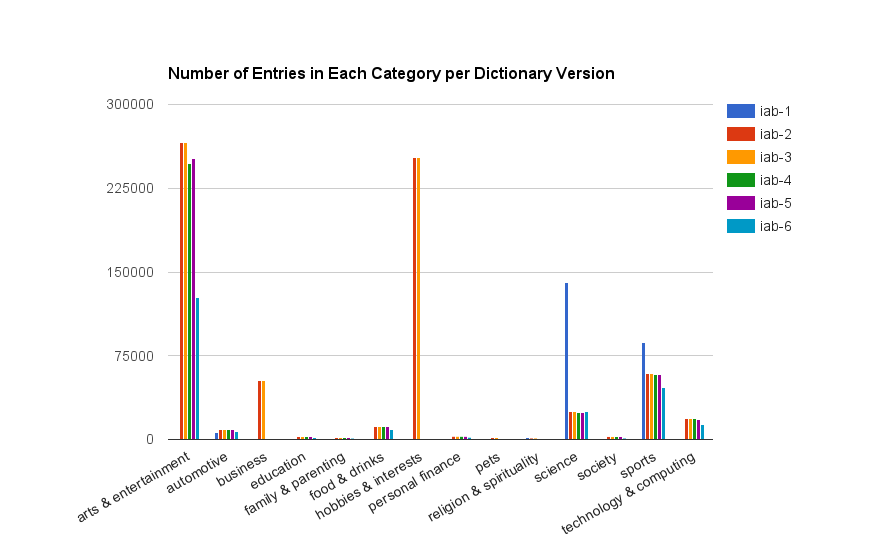
\includegraphics[width=\textwidth]{Chapters/Results/Numberofentriespercat}
\caption[Number of entries per category for each dictionary version]{Number of entries per category for each of our dictionary versions. Notice that not all categories are present in all versions.}
\label{fig:numberofentriespercat}
\end{figure}

\begin{comment}
We noticed that not all ambiguous entries were removed from the dictionary in version \emph{iab-5}. Thus, we collected all ambiguous category articles which are found under the category \emph{All ambiguous pages} (a total of *** pages). 




\end{comment}

\begin{table}[h]
\centering
\renewcommand{\arraystretch}{1.25}
\begin{tabular}{l|l|l|l|l|l|l}
                                & {\bf iab-1} & {\bf iab-2} & {\bf iab-3} & {\bf iab-4} & {\bf iab-5} & \textbf{iab-6} \\ \hline
{\bf arts \& entertainment}     &             & X           & X           & X           & X & X       \\ \hline
{\bf automotive}                & X           & X           & X           & X           & X & X       \\ \hline
{\bf business}                  &             & X           & X           &             &   &         \\ \hline
{\bf education}                 &             & X           & X           & X           &   &         \\ \hline
{\bf family \& parenting}       &             & X           & X           & X           & X & X       \\ \hline
{\bf food \& drinks}            &             & X           & X           & X           & X & X       \\ \hline
{\bf hobbies \& interests}      &             & X           & X           &             &   &         \\ \hline
{\bf personal finance}          &             & X           & X           & X           & X & X       \\ \hline
{\bf pets}                      &             & X           & X           &             &   &         \\ \hline
{\bf religion and spirituality} & X           & X           & X           &             &   &         \\ \hline
{\bf science}                   & X           & X           & X           & X           & X & X       \\ \hline
{\bf society}                   &             & X           & X           & X           & X & X       \\ \hline
{\bf sports}                    & X           & X           & X           & X           & X & X       \\ \hline
{\bf technology \& computing}   &             & X           & X           & X           & X & X       \\ 
\end{tabular}
\caption{Available categories for each dictionary version. }
\label{tab:available_categories}
\end{table}


\begin{comment}
Number of entries: 
iab-1: 693933
iab-2: 693933 ????
iab-3: 4487442
iab-4: 1141214
iab-5: 1153967
\end{comment}